\section{Quantum communication systems with squeezed states}
    In this section we assess the effect of squeezing on the performance in absence of photon 
    addition and thermal noise. The representation of squeezed states are given in \ref{squeezedStates}.
    As for PACS systems, it can be useful to define the mean 
    number of photon $n_p$ in a squeezed state, which is given by
    \begin{equation}
        n_p(\mu,r) = \absolutevalue{\mu}^2 + \left(\sinh{r}\right)^2;
    \end{equation}
    where $\mu$ is the amplitude of the starter coherent state and the squeezing factor
    is $\zeta = r e^{i\theta}$. The minimum value of $n_p$ is given by $n_p(0,r) = \sinh{r}^2$.

    \subsection{Quantum OOK}
    \begin{figure}[t]
        % This file was created by matlab2tikz.
%
%The latest updates can be retrieved from
%  http://www.mathworks.com/matlabcentral/fileexchange/22022-matlab2tikz-matlab2tikz
%where you can also make suggestions and rate matlab2tikz.
%
\definecolor{mycolor1}{rgb}{1.00000,0.00000,1.00000}%
\definecolor{mycolor2}{rgb}{0.00000,1.00000,1.00000}%
%
\begin{tikzpicture}

\begin{axis}[%
width=4.521in,
height=3.566in,
at={(0.758in,0.481in)},
scale only axis,
unbounded coords=jump,
xmin=0,
xmax=4,
xlabel style={font=\color{white!15!black}},
xlabel={$\bar{n}_p$},
ymode=log,
ymin=0.000952035382554339,
ymax=1,
yminorticks=true,
ylabel style={font=\color{white!15!black}},
ylabel={$P_e$},
axis background/.style={fill=white},
axis x line*=bottom,
axis y line*=left,
legend style={legend cell align=left, align=left, draw=white!15!black}
]
\addplot [color=red]
  table[row sep=crcr]{%
0	0.4996948239481\\
0.1	0.345757180805158\\
0.2	0.287121156846032\\
0.3	0.24545028417787\\
0.4	0.212911022589419\\
0.5	0.186364156125375\\
0.6	0.164146896047426\\
0.7	0.145241250969801\\
0.8	0.128963672155848\\
0.9	0.114827686582853\\
1	0.102469669846838\\
1.1	0.0916098861017105\\
1.2	0.0820267587705495\\
1.3	0.0735410565066186\\
1.4	0.0660058406114885\\
1.5	0.059298707245483\\
1.6	0.0533166878041113\\
1.7	0.0479720733113359\\
1.8	0.0431899288477867\\
1.9	0.0389056427143193\\
2	0.0350630885593494\\
2.1	0.0316133642448069\\
2.2	0.0285137165123738\\
2.3	0.0257264385174695\\
2.4	0.0232184857173818\\
2.5	0.0209604826478608\\
2.6	0.018926505879439\\
2.7	0.0170934733750665\\
2.8	0.015440858978732\\
2.9	0.0139503375508124\\
3	0.0126055969522582\\
3.1	0.0113920033292345\\
3.2	0.0102964976303588\\
3.3	0.00930735236679731\\
3.4	0.00841405465378259\\
3.5	0.00760715856948718\\
3.6	0.0068781912376874\\
3.7	0.00621951875544752\\
3.8	0.00562428411547444\\
3.9	0.00508630643116037\\
4	0.00460003679294951\\
};
\addlegendentry{r = 0}

\addplot [color=red, only marks, mark=o, mark options={solid, red}]
  table[row sep=crcr]{%
0	0.4996948239481\\
};
\addlegendentry{r = 0.01}

\addplot [color=red, only marks, mark=o, mark options={solid, red}]
  table[row sep=crcr]{%
0.5	0.4996948239481\\
};
\addlegendentry{r = 0.1}

\addplot [color=red, only marks, mark=o, mark options={solid, red}]
  table[row sep=crcr]{%
1	0.4996948239481\\
};
\addlegendentry{r = 0.2}

\addplot [color=red, only marks, mark=o, mark options={solid, red}]
  table[row sep=crcr]{%
1.5	0.4996948239481\\
};
\addlegendentry{r = 0.5}

\addplot [color=red, only marks, mark=o, mark options={solid, red}, forget plot]
  table[row sep=crcr]{%
2	0.4996948239481\\
};
\addplot [color=red, only marks, mark=o, mark options={solid, red}, forget plot]
  table[row sep=crcr]{%
2.5	0.4996948239481\\
};
\addplot [color=red, only marks, mark=o, mark options={solid, red}, forget plot]
  table[row sep=crcr]{%
3	0.4996948239481\\
};
\addplot [color=red, only marks, mark=o, mark options={solid, red}, forget plot]
  table[row sep=crcr]{%
3.5	0.4996948239481\\
};
\addplot [color=red, only marks, mark=o, mark options={solid, red}, forget plot]
  table[row sep=crcr]{%
4	0.4996948239481\\
};
\addplot [color=green, forget plot]
  table[row sep=crcr]{%
0	nan\\
0.1	0.345064018736899\\
0.2	0.286187372245113\\
0.3	0.244381641821762\\
0.4	0.211763047105019\\
0.5	0.185173064834948\\
0.6	0.162937642185644\\
0.7	0.144031757964237\\
0.8	0.127767275529543\\
0.9	0.113654069132882\\
1	0.10132632364131\\
1.1	0.0905020842185692\\
1.2	0.0809582894225724\\
1.3	0.0725146416016301\\
1.4	0.0650232396075375\\
1.5	0.0583608166530484\\
1.6	0.0524237219713765\\
1.7	0.0471239463376132\\
1.8	0.0423861549024593\\
1.9	0.0381452869835203\\
2	0.0343451214923461\\
2.1	0.03093645129925\\
2.2	0.0278764546767297\\
2.3	0.0251273768898007\\
2.4	0.0226560519684494\\
2.5	0.0204330668185038\\
2.6	0.0184324797606132\\
2.7	0.0166312087814519\\
2.8	0.0150087416267342\\
2.9	0.0135467790137929\\
3	0.0122290428253946\\
3.1	0.0110409651304977\\
3.2	0.00996948449447915\\
3.3	0.00900297076544082\\
3.4	0.00813092412607835\\
3.5	0.00734397700992612\\
3.6	0.00663371401765406\\
3.7	0.00599257358816813\\
3.8	0.0054137275868128\\
3.9	0.00489107971825575\\
4	0.004419112867945\\
};
\addplot [color=green, only marks, mark=square, mark options={solid, green}, forget plot]
  table[row sep=crcr]{%
0	nan\\
};
\addplot [color=green, only marks, mark=square, mark options={solid, green}, forget plot]
  table[row sep=crcr]{%
0.5	nan\\
};
\addplot [color=green, only marks, mark=square, mark options={solid, green}, forget plot]
  table[row sep=crcr]{%
1	nan\\
};
\addplot [color=green, only marks, mark=square, mark options={solid, green}, forget plot]
  table[row sep=crcr]{%
1.5	nan\\
};
\addplot [color=green, only marks, mark=square, mark options={solid, green}, forget plot]
  table[row sep=crcr]{%
2	nan\\
};
\addplot [color=green, only marks, mark=square, mark options={solid, green}, forget plot]
  table[row sep=crcr]{%
2.5	nan\\
};
\addplot [color=green, only marks, mark=square, mark options={solid, green}, forget plot]
  table[row sep=crcr]{%
3	nan\\
};
\addplot [color=green, only marks, mark=square, mark options={solid, green}, forget plot]
  table[row sep=crcr]{%
3.5	nan\\
};
\addplot [color=green, only marks, mark=square, mark options={solid, green}, forget plot]
  table[row sep=crcr]{%
4	nan\\
};
\addplot [color=blue, forget plot]
  table[row sep=crcr]{%
0	nan\\
0.1	0.342911242050718\\
0.2	0.28058961140917\\
0.3	0.237013615624501\\
0.4	0.203362627785208\\
0.5	0.176172423921015\\
0.6	0.153621129473415\\
0.7	0.134598552001024\\
0.8	0.118361111210907\\
0.9	0.104380130690808\\
1	0.0922620419252684\\
1.1	0.0817039223529157\\
1.2	0.0724666945589215\\
1.3	0.0643575588674198\\
1.4	0.0572190562504042\\
1.5	0.0509203137421171\\
1.6	0.0453515615989874\\
1.7	0.0404200410126793\\
1.8	0.036046499652801\\
1.9	0.0321631768342768\\
2	0.0287114380592102\\
2.1	0.0256404630750137\\
2.2	0.0229061115233933\\
2.3	0.0204696999940017\\
2.4	0.0182975075201901\\
2.5	0.0163597742310368\\
2.6	0.0146303978697211\\
2.7	0.0130863360990972\\
2.8	0.0117072108830385\\
2.9	0.0104750164931909\\
3	0.00937374288410803\\
3.1	0.00838926633942438\\
3.2	0.00750897215726454\\
3.3	0.00672168429436226\\
3.4	0.00601744615112698\\
3.5	0.00538739392489546\\
3.6	0.004823640184214\\
3.7	0.0043191402885786\\
3.8	0.00386760371936712\\
3.9	0.00346344111948527\\
4	0.00310164723719591\\
};
\addplot [color=blue, only marks, mark=triangle, mark options={solid, blue}, forget plot]
  table[row sep=crcr]{%
0	nan\\
};
\addplot [color=blue, only marks, mark=triangle, mark options={solid, blue}, forget plot]
  table[row sep=crcr]{%
0.5	nan\\
};
\addplot [color=blue, only marks, mark=triangle, mark options={solid, blue}, forget plot]
  table[row sep=crcr]{%
1	nan\\
};
\addplot [color=blue, only marks, mark=triangle, mark options={solid, blue}, forget plot]
  table[row sep=crcr]{%
1.5	nan\\
};
\addplot [color=blue, only marks, mark=triangle, mark options={solid, blue}, forget plot]
  table[row sep=crcr]{%
2	nan\\
};
\addplot [color=blue, only marks, mark=triangle, mark options={solid, blue}, forget plot]
  table[row sep=crcr]{%
2.5	nan\\
};
\addplot [color=blue, only marks, mark=triangle, mark options={solid, blue}, forget plot]
  table[row sep=crcr]{%
3	nan\\
};
\addplot [color=blue, only marks, mark=triangle, mark options={solid, blue}, forget plot]
  table[row sep=crcr]{%
3.5	nan\\
};
\addplot [color=blue, only marks, mark=triangle, mark options={solid, blue}, forget plot]
  table[row sep=crcr]{%
4	nan\\
};
\addplot [color=mycolor1, forget plot]
  table[row sep=crcr]{%
0	nan\\
0.1	0.352483179556453\\
0.2	0.282015320063401\\
0.3	0.234732372951055\\
0.4	0.198938618050338\\
0.5	0.170422220223627\\
0.6	0.147047605722407\\
0.7	0.12753619551938\\
0.8	0.111045202459609\\
0.9	0.0969796510639878\\
1	0.0849000679635937\\
1.1	0.0744706800960189\\
1.2	0.0654275840690521\\
1.3	0.0575597358535224\\
1.4	0.0506950380305154\\
1.5	0.0446916628730589\\
1.6	0.0394311481668558\\
1.7	0.0348141620942864\\
1.8	0.030756195940998\\
1.9	0.0271853117419146\\
2	0.0240397830099432\\
2.1	0.0212665456031397\\
2.2	0.0188196302835341\\
2.3	0.0166592253798481\\
2.4	0.0147506425523341\\
2.5	0.0130637022853067\\
2.6	0.0115720329348848\\
2.7	0.0102524759571693\\
2.8	0.00908478476977853\\
2.9	0.00805119723079872\\
3	0.00713606551874252\\
3.1	0.00632562120224001\\
3.2	0.00560774441838796\\
3.3	0.00497174792321697\\
3.4	0.00440820528309399\\
3.5	0.00390878880218942\\
3.6	0.00346615989599225\\
3.7	0.00307380367294957\\
3.8	0.00272598065309104\\
3.9	0.00241761535472995\\
4	0.00214420611137395\\
};
\addplot [color=mycolor1, only marks, mark=diamond, mark options={solid, mycolor1}, forget plot]
  table[row sep=crcr]{%
0	nan\\
};
\addplot [color=mycolor1, only marks, mark=diamond, mark options={solid, mycolor1}, forget plot]
  table[row sep=crcr]{%
0.5	nan\\
};
\addplot [color=mycolor1, only marks, mark=diamond, mark options={solid, mycolor1}, forget plot]
  table[row sep=crcr]{%
1	nan\\
};
\addplot [color=mycolor1, only marks, mark=diamond, mark options={solid, mycolor1}, forget plot]
  table[row sep=crcr]{%
1.5	nan\\
};
\addplot [color=mycolor1, only marks, mark=diamond, mark options={solid, mycolor1}, forget plot]
  table[row sep=crcr]{%
2	nan\\
};
\addplot [color=mycolor1, only marks, mark=diamond, mark options={solid, mycolor1}, forget plot]
  table[row sep=crcr]{%
2.5	nan\\
};
\addplot [color=mycolor1, only marks, mark=diamond, mark options={solid, mycolor1}, forget plot]
  table[row sep=crcr]{%
3	nan\\
};
\addplot [color=mycolor1, only marks, mark=diamond, mark options={solid, mycolor1}, forget plot]
  table[row sep=crcr]{%
3.5	nan\\
};
\addplot [color=mycolor1, only marks, mark=diamond, mark options={solid, mycolor1}, forget plot]
  table[row sep=crcr]{%
4	nan\\
};
\addplot [color=mycolor2, forget plot]
  table[row sep=crcr]{%
0	nan\\
0.1	nan\\
0.2	nan\\
0.3	0.306786766345818\\
0.4	0.242590630097618\\
0.5	0.197918895572083\\
0.6	0.164073400870317\\
0.7	0.137366478836737\\
0.8	0.115784377573039\\
0.9	0.0980699796818669\\
1	0.0833714751942309\\
1.1	0.0710774586522101\\
1.2	0.0607327341300646\\
1.3	0.0519875094320926\\
1.4	0.0445671089158063\\
1.5	0.0382519606700177\\
1.6	0.0328646519862905\\
1.7	0.0282596802292375\\
1.8	0.0243169681921276\\
1.9	0.0209367128708955\\
2	0.0180353163612855\\
2.1	0.0155426264094213\\
2.2	0.013399252202812\\
2.3	0.0115550198413198\\
2.4	0.00996724028084983\\
2.5	0.00859955485624092\\
2.6	0.00742097560285826\\
2.7	0.00640497624240516\\
2.8	0.0055288612502285\\
2.9	0.0047731718879836\\
3	0.00412119408203854\\
3.1	0.00355860194225149\\
3.2	0.00307303906910844\\
3.3	0.00265391333494414\\
3.4	0.00229208259247371\\
3.5	0.00197968020442113\\
3.6	0.00170993158525734\\
3.7	0.00147699358221837\\
3.8	0.00127582696954853\\
3.9	0.00110208961226266\\
4	0.000952035382554339\\
};
\addplot [color=mycolor2, only marks, mark=star, mark options={solid, mycolor2}, forget plot]
  table[row sep=crcr]{%
0	nan\\
};
\addplot [color=mycolor2, only marks, mark=star, mark options={solid, mycolor2}, forget plot]
  table[row sep=crcr]{%
0.5	nan\\
};
\addplot [color=mycolor2, only marks, mark=star, mark options={solid, mycolor2}, forget plot]
  table[row sep=crcr]{%
1	nan\\
};
\addplot [color=mycolor2, only marks, mark=star, mark options={solid, mycolor2}, forget plot]
  table[row sep=crcr]{%
1.5	nan\\
};
\addplot [color=mycolor2, only marks, mark=star, mark options={solid, mycolor2}, forget plot]
  table[row sep=crcr]{%
2	nan\\
};
\addplot [color=mycolor2, only marks, mark=star, mark options={solid, mycolor2}, forget plot]
  table[row sep=crcr]{%
2.5	nan\\
};
\addplot [color=mycolor2, only marks, mark=star, mark options={solid, mycolor2}, forget plot]
  table[row sep=crcr]{%
3	nan\\
};
\addplot [color=mycolor2, only marks, mark=star, mark options={solid, mycolor2}, forget plot]
  table[row sep=crcr]{%
3.5	nan\\
};
\addplot [color=mycolor2, only marks, mark=star, mark options={solid, mycolor2}, forget plot]
  table[row sep=crcr]{%
4	nan\\
};
\end{axis}

\begin{axis}[%
width=5.833in,
height=4.375in,
at={(0in,0in)},
scale only axis,
xmin=0,
xmax=1,
ymin=0,
ymax=1,
axis line style={draw=none},
ticks=none,
axis x line*=bottom,
axis y line*=left
]
\end{axis}
\end{tikzpicture}%
        \caption{MDEP of OOK squeezed states system as function of $\bar{n}_p$ without thermal 
        noise, $N=45$, $\theta=\pi$ and equiprobable symbols.}
        \label{fig:OOK_SS}
    \end{figure}
    A quantum OOK system with squeezed states is a system with the following constellation
    \begin{subequations}
        \begin{align}
            \Operator{\varXi}_0 &= \Operator{\varXi}(0,0)\\
            \Operator{\varXi}_1 &= \Operator{\varXi}(\mu,\zeta)
        \end{align}
    \end{subequations}
    where $\Operator{\varXi}_{\mathrm{th}}(\mu,\zeta)$ is the squeezed state with amplitude $\mu$
    and squeezing parameter $\zeta$.

    The MDEP as function of $\bar{n}_p$,
    i.e the mean number of photon in the system,  is plotted in figure \ref{fig:OOK_SS} with:
    $\theta=\pi$, $N=45$, equiprobable symbols and $\bar{n}=0$.
    It can be noticed that the optimal configuration of $r$ depends on the energy in the 
    system. For low energy levels the squeezing has not a positive effect.
    \subsection{Quantum BPSK}
    The effect of the squeezing in a BPSK system is similar to that in the OOK. The constellation
    of this type of system is given by
    \begin{subequations}
        \begin{align}
            \Operator{\varXi}_0 &= \Operator{\varXi}(-\mu,\zeta)\\
            \Operator{\varXi}_1 &= \Operator{\varXi}(\mu,\zeta).
        \end{align}
    \end{subequations}
    Figure \ref{fig:3.5} shows the MDEP of the system as function of $\bar{n}_p$
    with $\theta=\pi$, $N=45$, equiprobable symbols and $\bar{n}=0$.

    \begin{figure}[t]
        \begin{center}
            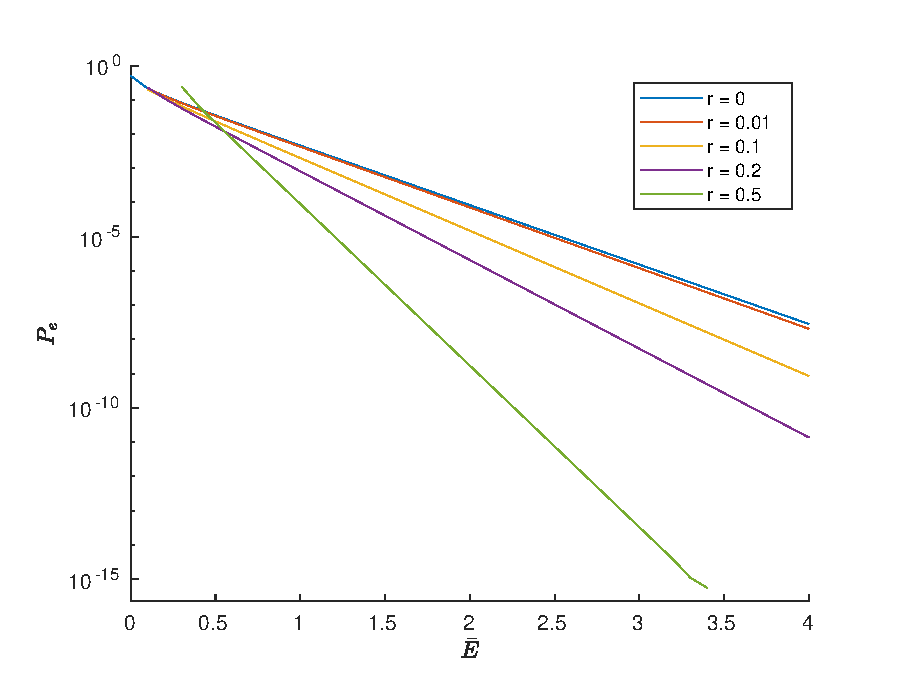
\includegraphics[width=0.8\textwidth]{fig3.5.eps}
            \caption{MDEP of squeezed state BPSK system as function of $\bar{n}_p$. 
                $N=30$, $\bar{n}=0$, $\theta=\pi$, $p_0=p_1=1/2$}
            \label{fig:3.5}
        \end{center}     
    \end{figure}